\documentclass[11pt]{article}
% Adapted from an original template by Hlyni Arnórssyni,
% Reykjavik University, Iceland

% pgfplots loads xcolor first, so pass the table option early to avoid an option clash.
\PassOptionsToPackage{table}{xcolor}

% ------------------------------ PAGE SETTINGS ------------------------------
\usepackage{geometry}

\geometry{
    paper=a4paper,
    top=2.5cm,
    bottom=2.5cm,
    left=2.5cm,
    right=2.4cm,
    headheight=0.75cm,
    footskip=1.5cm,
    headsep=0.75cm
}

% ------------------------------ BASIC PACKAGES ------------------------------
\usepackage{blindtext}

% Character encoding
\usepackage[T1]{fontenc}
\usepackage[utf8]{inputenc}

% Mathematics
\usepackage{amsmath, amsfonts, amsthm, amssymb}
\usepackage{braket, nicefrac}

% SI units
\usepackage{siunitx}

% Lists / columns
\usepackage{enumitem, multicol}

% ------------------------------ FIGURES ------------------------------
\usepackage{graphicx}
\usepackage{float}
\usepackage{keystroke}
\usepackage{pgfplots}
\usepgfplotslibrary{units}
\pgfplotsset{compat=1.16}

% Search these locations automatically for figures
\graphicspath{{fig/}{graphics/}{Graphics/}{./}}

% ------------------------------ TABLES ------------------------------
\usepackage{tabularx}
\usepackage{array}
\usepackage[table]{xcolor}

% ------------------------------ TYPOGRAPHY ------------------------------
\usepackage{caption}
\usepackage{titlesec}
\usepackage{microtype}
\usepackage{csquotes}

% ------------------------------ COLORS ------------------------------
\definecolor{GWBlue}{HTML}{1E4E79}

% ------------------------------ SECTION STYLING ------------------------------
\titleformat{\section}
  {\Large\bfseries\color{GWBlue}}
  {\thesection.}
  {0.40em}
  {}

\titlespacing*{\section}
  {0pt}
  {0.70em}
  {0.28em}

% ------------------------------ CAPTION STYLING ------------------------------
\captionsetup{
    font=small,
    labelfont=bf,
    textfont=it,
    labelsep=period,
    skip=4pt
}

% ------------------------------ PARAGRAPH SPACING ------------------------------
\setlength{\parindent}{0pt}
\setlength{\parskip}{0.30em}

% ------------------------------ BIBLIOGRAPHY ------------------------------
\usepackage[
    backend=biber,
    style=authoryear,
    sorting=none,
    giveninits=true,
    maxbibnames=99,
    dashed=false
]{biblatex}

\addbibresource{references.bib}

\DeclareNameAlias{sortname}{family-given}
\DeclareNameAlias{default}{family-given}
\DeclareFieldFormat[article]{title}{#1}
\DeclareFieldFormat[misc]{title}{#1}
\renewbibmacro{in:}{}

\AtEveryBibitem{%
    \clearfield{doi}%
    \clearfield{urldate}%
}

\AtBeginBibliography{\small}
\setlength{\bibitemsep}{0.35em}

% ------------------------------ HYPERLINKS ------------------------------
\usepackage{hyperref}

\hypersetup{
    colorlinks=true,
    linkcolor=GWBlue,
    citecolor=GWBlue,
    urlcolor=GWBlue
}
\usetikzlibrary{arrows.meta,positioning,fit,backgrounds}
\newcolumntype{C}[1]{>{\centering\arraybackslash}p{#1}}

\begin{document}

\begin{center}

\includegraphics[width=0.28\textwidth]{gwu_logo.pdf}\par\vspace{4pt}
{\Large\bfseries Where Do Neural Networks Fail? Fashion-MNIST\par}
{\large\bfseries Post-Training Analysis and Novelty Detection Using\\ Neural Network Self-Organizing Maps (NNSOM)\par}
\vspace{6pt}
{\normalsize Capstone Group 5: Fyrooz Anika Khan, Nazish Atta\par}
{\small DATS 6501 Capstone, Fall 2026, The George Washington University. Supervised by Dr.\ Amir Jafari.\par}
\end{center}

\begin{abstract}
\noindent We repeat our MNIST study on Fashion-MNIST, a harder dataset of clothing images, with every step and rule copied unchanged. A LeNet-5 reaches 90.90\% test accuracy, about ten times as many mistakes as on MNIST. On a 15$\times$15 self-organizing map (SOM) trained on its internal features, the classes form regions (89.3\% purity against 17.3\% by chance), and the mistakes gather in 11 cells that hold 3.9 times their fair share, inside one broad region where the upper-body garments overlap. A k-means grouping finds the mistakes as well as the SOM (AUROC 0.812 against 0.811), and the CNN's own confidence does better (0.906).
As a novelty detector, the SOM's quantization error separates SVHN images from Fashion-MNIST only weakly (AUROC 0.789; energy 0.982), and its fixed alarm catches fewer SVHN images than normal ones. On clothing classes the CNN never saw, however, the SOM beats the CNN's confidence in all five class splits (+0.046 AUROC).
Used to guide retraining, SOM-chosen hard images with altered copies did not clearly lower the mistakes in the error cells (36.0\% to 34.0\%, interval includes 0), unlike on MNIST, and curriculum learning made the CNN clearly worse. New SOMs after retraining are not purer, and SOM-guided retraining lowered the map's novelty AUROC. Every result is compared with a control or a chance level.
\par\smallskip
\noindent\textbf{Keywords:} self-organizing map, post-training analysis, error analysis, novelty detection, Fashion-MNIST.
\end{abstract}

\section{Introduction}

On MNIST our LeNet-5 \parencite{lecun1998gradient} was right 99\% of the time, which left only 86 test mistakes to study and very little room for retraining to help. Fashion-MNIST \parencite{xiao2017fashion} has the same format (70,000 grey $28\times28$ images, 10 classes) but shows clothing, and the same network gets only 90.90\% of the test images right (956 mistakes in 10,500 images).
The question stays the same: where do the mistakes come from, and can a map of the network's features help?

Tools such as saliency maps \parencite{simonyan2014saliency}, LIME \parencite{ribeiro2016lime} and SHAP \parencite{lundberg2017shap} explain one prediction at a time. We use a Self-Organizing Map (SOM) \parencite{kohonen1990som}, through the NNSOM library \parencite{jafari_nnsom}, to see where in the network's features the mistakes gather.
We train the CNN, record the 84 numbers it computes for each image just before it answers (the \emph{embedding}), and train a SOM on them. We ask the same three questions as for MNIST:
(i)~where on the map do the CNN's mistakes gather; (ii)~can the map spot inputs that are unlike the training data; and (iii)~can the map choose better samples for retraining than random choice?
Every step, setting and success criterion is the MNIST one, written down in the Fashion-MNIST protocol before any Fashion-MNIST data was loaded; the few changes the dataset forced are stated where they apply.

\textbf{Contributions.}
(1)~The MNIST pipeline run unchanged on a harder dataset, so the two can be compared directly.
(2)~Evidence that the CNN's mistakes gather where whole classes overlap, tested against chance on three grid sizes.
(3)~A comparison with simple baselines, which again shows that the pattern is not special to the SOM and that the CNN's confidence finds mistakes better.
(4)~Tests of the SOM as a novelty detector (far novelty with SVHN, near novelty with unseen clothing classes) and as a guide for retraining. On Fashion-MNIST the SOM wins one test it did not win on MNIST (unseen classes) and loses one it won (guided retraining).

\section{Related Work}

The related work is the same as for the MNIST study; we summarize it and say how this report differs.

\textbf{CNNs as a source of features.} LeNet-5 \parencite{lecun1998gradient} trained with Adam \parencite{kingma2015adam} is our fixed network. Fashion-MNIST \parencite{xiao2017fashion} was made as a harder drop-in replacement for MNIST, which is why we use it as the second dataset.

\textbf{Explaining single predictions.} Saliency maps \parencite{simonyan2014saliency}, LIME \parencite{ribeiro2016lime} and SHAP \parencite{lundberg2017shap} answer ``why this prediction?''. We ask ``where in the network's features do mistakes gather?''.

\textbf{Self-Organizing Maps.} Kohonen's SOM \parencite{kohonen1990som} keeps similar data in nearby cells; Vesanto and Alhoniemi \parencite{vesanto2000clustering} measure how the cells group. SOM-VAE \parencite{fortuin2019somvae} and DESOM \parencite{forest2021desom} train features and map together; we keep the CNN fixed so the map can be judged on its own.

\textbf{Finding systematic errors.} Domino \parencite{eyuboglu2022domino} and the Spotlight \parencite{deon2022spotlight} search for groups or regions where a model does badly. We use one fixed, readable map and test every claim against chance and simple baselines.

\textbf{Novelty detection.} Max-softmax \parencite{hendrycks2017baseline}, ODIN \parencite{liang2018odin}, Mahalanobis distance \parencite{lee2018mahalanobis}, energy \parencite{liu2020energy}, Deep SVDD \parencite{ruff2018deep} and nearest-neighbour distance \parencite{sun2022knn} are surveyed by Yang et al.\ \parencite{yang2024generalized}. We also compare Isolation Forest \parencite{liu2008isolation}, the One-Class SVM \parencite{scholkopf2001support} and an autoencoder \parencite{sakurada2014autoencoder}. Nalisnick et al.\ \parencite{nalisnick2019deep} showed that models of normal data can rate SVHN as more typical, which we see again. For unseen classes we follow the open-set protocol of Neal et al.\ \parencite{neal2018open}, where max-softmax is a strong baseline \parencite{vaze2022openset}.

\textbf{How this report differs.} It is a replication: the same design on a dataset where the network makes ten times as many mistakes. That changes several conclusions, and the comparison with MNIST (Table~\ref{tab:mnist}) is part of the result.

\section{Method}
\label{sec:method}

\subsection{Data and model}

Fashion-MNIST is split once into 49,000 training, 10,500 validation and 10,500 test images, with the same share of each class in every part and a fixed random seed. The ten classes are T-shirt/top, Trouser, Pullover, Dress, Coat, Sandal, Shirt, Sneaker, Bag and Ankle boot.
We train a LeNet-5 with the MNIST recipe (Adam, 20 epochs, learning rate $\times0.1$ every 10 epochs, seed 42) and keep the epoch with the best validation accuracy (epoch 16). For every image we record the 84 numbers of the second-to-last layer (fc2), the embedding, and rescale them to $-1$ to $1$ using the training data only (Figure~\ref{fig:pipeline}).

\begin{figure}[H]
\centering
\begin{tikzpicture}[
  font=\scriptsize, node distance=5mm and 4mm,
  box/.style={draw=GWBlue, rounded corners=2pt, align=center, minimum height=10mm, text width=30mm, fill=GWBlue!6, line width=0.6pt},
  tag/.style={font=\bfseries\scriptsize, text=GWBlue, anchor=south west, inner sep=1pt},
  arr/.style={-{Stealth[length=2mm]}, line width=0.6pt, draw=GWBlue}]
\node[box] (data) {Fashion-MNIST\\70,000 images};
\node[box, right=of data] (split) {Stratified split\\49,000 / 10,500 / 10,500};
\node[box, right=of split] (cnn) {Baseline LeNet-5\\90.90\% test accuracy};
\node[box, right=of cnn] (emb) {fc2 embeddings\\84 dimensions};
\node[tag] at (data.north west) {Phase 1: Model Training Baseline};
\node[box, below=9mm of emb] (som) {SOM training\\NNSOM 15$\times$15};
\node[box, left=of som] (viz) {SOM visualization\\U-matrix, hit histogram};
\node[box, left=of viz] (cluster) {Cluster analysis\\purity, class overlap};
\node[box, left=of cluster] (err) {Error pattern analysis\\hotspots, baseline checks};
\node[tag] at (err.north west) {Phase 2: SOM Training and Visualization};
\node[box, below=9mm of err] (nov) {Novelty detection\\SVHN, unseen classes};
\node[box, right=of nov] (cmp) {Comparative evaluation\\max-softmax, energy, Mahalanobis, \dots};
\node[box, right=of cmp] (retrain) {Guided retraining\\hard examples, augmentation};
\node[box, right=of retrain] (rean) {Iterative SOM re-analysis\\before / after};
\node[tag, anchor=north west] at (nov.south west) {Phases 3 and 4};
\draw[arr] (data) -- (split); \draw[arr] (split) -- (cnn); \draw[arr] (cnn) -- (emb);
\draw[arr] (emb) -- (som); \draw[arr] (som) -- (viz); \draw[arr] (viz) -- (cluster); \draw[arr] (cluster) -- (err);
\draw[arr] (err) -- (nov); \draw[arr] (nov) -- (cmp);
\draw[arr] (cmp) -- (retrain); \draw[arr] (retrain) -- (rean);
\end{tikzpicture}
\caption{The project pipeline on Fashion-MNIST, the same as for MNIST: the baseline CNN (Phase 1), the SOM (Phase 2), novelty detection (Phase 3) and guided retraining with a new SOM (Phase 4).}
\label{fig:pipeline}
\end{figure}

\subsection{Self-Organizing Map}

We train a 15$\times$15 map (225 cells) on the 49,000 training embeddings with NNSOM's batch rule (250 epochs, starting neighbourhood radius 11, seed 42). Each image is assigned to its closest cell, its best-matching neuron (BMU).
The quantization error (QE) is the average distance between an image and its cell; the topological error (TE1) is the share of images whose two closest cells are not grid neighbours.

The grid size was tested with MNIST's pre-registered comparison: three grids (10$\times$10, 15$\times$15, 20$\times$20), ten maps each, and each cell's error rate on half of the validation images used to predict the mistakes on the other half, over 200 splits.
Larger grids fit more closely (QE 1.054, 0.913 and 0.844) and are slightly purer (87.9\%, 89.0\% and 89.5\%), but have a higher topological error (TE1 4.8\%, 6.3\% and 7.7\%).
Unlike on MNIST, the comparison is decided: \textbf{15$\times$15 predicts the mistakes better than 20$\times$20} (AUROC difference $-0.042$ for 20$\times$20, 95\% range $-0.077$ to $-0.008$), and 15$\times$15 and 10$\times$10 cannot be told apart. With 876 validation mistakes instead of 92, the ranges are about three times narrower.
A check with 20 Optuna \parencite{akiba2019optuna} trials per grid found no setting better on both QE and TE1, and a feature-layer check showed that maps on fc2 find mistakes better than maps on the earlier fc1 layer in all 5 SOM seeds (AUROC $-0.055$ for fc1).

\subsection{Finding where mistakes gather}

For each cell we compute its \emph{purity} (the share of its images that belong to its most common class) and the \emph{entropy} of its class mix, and compare the overall purity with 1,000 label shuffles.
Hotspots are the $\max(5,\,5\%\text{ of the cells})$ cells with the highest lower end of the 95\% Wilson interval \parencite{wilson1927probable} of their error rate, picked on a random half of the validation images and measured on the other half with the \emph{concentration ratio}:
\[
\text{ratio}=\frac{\text{share of the mistakes that fall in hotspots}}{\text{share of the images that fall in hotspots}},
\]
over 200 half-splits, against 200 shuffles of the mistake labels. We also compute the Spearman correlation between a cell's error rate and its purity and entropy.

\subsection{Comparison with simple baselines}

As for MNIST: (a)~k-means with 225 clusters; (b)~the impurity of the 15 nearest training embeddings; and (c)~the network's maximum softmax probability \parencite{hendrycks2017baseline}. Each score is judged by AUROC on the same validation images, and in a same-budget check every method may flag the same share of images as the SOM's hotspots.

\subsection{Phase 3: Novelty detection}

The CNN and SOM stay fixed. \textbf{Far novelty:} the 10,500 Fashion-MNIST validation images are normal and the 26,032 SVHN test images \parencite{netzer2011reading} (house-number photographs, the same images as for MNIST) are novel.
The SOM gives two scores, QE and the U-matrix score; we compare them with max-softmax, energy \parencite{liu2020energy}, Mahalanobis \parencite{lee2018mahalanobis}, nearest-neighbour distance \parencite{sun2022knn}, Isolation Forest, One-Class SVM and an autoencoder, all on the same embeddings, by AUROC \parencite{fawcett2006roc}, AUPR \parencite{saito2015pr} and the false-positive rate at 95\% TPR. The QE alarm threshold is the 95th percentile of the training QE (1.4215), fixed in advance.
\textbf{Near novelty:} in 5 class splits a new network and map are trained on 6 classes and tested on the other 4 \parencite{neal2018open}. The statements (for example ``QE is better than max-softmax'') and their decision rules were fixed before any Fashion-MNIST novelty score existed.

\subsection{Phase 4: Guided retraining}

The retraining design is MNIST's (Figure~\ref{fig:loop}): the Phase 1 recipe, 5 seeds with the same seeds for every method, training images only.
A training image is \emph{hard} if its cell is one of the 11 error hotspots, or its cell has a purity below 0.95, or it lies above the 95th percentile of the distance to its cell. On Fashion-MNIST this pool holds 19,997 of the 49,000 training images (40.8\%; MNIST 8.6\%), because many cells are mixed.
In \emph{curriculum learning} the CNN starts with the easy images plus 10\% of the hard pool, with 10\% more every 5 epochs. In \emph{targeted augmentation} we add three altered copies of every hard image. Controls use the same number of images: random images with the same class mix, the least-confident images, and gradual versions.
One change was forced by the dataset: MNIST's augmentation ranges failed the check made before training (the Phase 1 network's validation accuracy fell from 91.66\% to 83.60\% on the altered images, limit 2 points), because clothing fills the $28\times28$ frame and turns and zooms cut off sleeves and hems. By a rule written down first, all ranges were halved twice (rotation 2.5$^\circ$, shift 0.25 pixel, zoom 0.975 to 1.025, shear 2$^\circ$), which passed (90.46\%).
The success criteria (A1, the primary one: SOM-chosen copies beat random copies on the hotspot test images) and the macro-F1 guard (0.0033, measured by MNIST's rule) were stamped before the test images were used, once.

\begin{figure}[H]
\centering
\begin{tikzpicture}[
  font=\scriptsize, node distance=9mm,
  box/.style={draw=GWBlue, rounded corners=2pt, align=center, minimum height=11mm, minimum width=38mm, fill=GWBlue!6, line width=0.6pt},
  arr/.style={-{Stealth[length=2mm]}, line width=0.7pt, draw=GWBlue}]
\node[box] (a) {\textbf{1. SOM analysis}\\ 11 hotspot cells,\\ 19,997 hard images};
\node[box, right=of a] (b) {\textbf{2. Targeted retraining}\\ curriculum or\\ augmented copies};
\node[box, right=of b] (c) {\textbf{3. New SOMs}\\ trained on the retrained\\ CNNs (15 maps)};
\draw[arr] (a)--(b); \draw[arr] (b)--(c);
\draw[arr, dashed] (c.south) -- ++(0,-6mm) -| (a.south);
\end{tikzpicture}
\caption{The feedback loop of Phase 4. The dashed arrow marks a next round, which we did not run.}
\label{fig:loop}
\end{figure}

After retraining, a new 15$\times$15 SOM is trained on each retrained CNN (standard, SOM-guided and random augmentation, 5 seeds each) and measured on validation images: purity, topological error and the error rate in each map's 11 worst cells. Each retrained network is also tested again against SVHN. The statements about the new maps and the novelty test were fixed before these runs.

\subsection{End-to-end comparison}

Two paths are compared on the same test images (Figure~\ref{fig:endtoend}): in path~1 (CF1) an image goes through the CNN; in path~2 (CF2) the CNN has first been retrained with SOM-guided augmentation. For a fair comparison CF1 is the five-seed average of the \emph{standard} retraining arm (90.66\% test accuracy, against 90.90\% for the single Phase 1 model), so any difference comes from the SOM guidance.

\begin{figure}[H]
\centering
\begin{tikzpicture}[
  font=\scriptsize, node distance=6mm,
  box/.style={draw=GWBlue, rounded corners=2pt, align=center, minimum height=9mm, minimum width=19mm, fill=GWBlue!6, line width=0.6pt},
  som/.style={box, dashed, fill=white},
  cf/.style={draw=GWBlue, fill=white, minimum width=22mm, minimum height=14mm, align=center, line width=0.6pt},
  arr/.style={-{Stealth[length=2mm]}, line width=0.6pt, draw=GWBlue}]
\node[box] (s1) {Sample};
\node[box, right=of s1] (c1) {CNN};
\node[box, right=of c1] (p1) {Prediction};
\node[cf, right=of p1] (m1) {CF1\\confusion matrix\\(as in Phase 1)};
\node[box, below=14mm of s1] (s2) {Sample};
\node[som, right=of s2] (g2) {SOM-guided\\retraining};
\node[box, right=of g2] (c2) {CNN};
\node[box, right=of c2] (p2) {Prediction};
\node[cf, right=of p2] (m2) {CF2\\confusion matrix\\(after retraining)};
\draw[arr] (s1)--(c1); \draw[arr] (c1)--(p1); \draw[arr] (p1)--(m1);
\draw[arr] (s2)--(g2); \draw[arr] (g2)--(c2); \draw[arr] (c2)--(p2); \draw[arr] (p2)--(m2);
\node[font=\bfseries\scriptsize, text=GWBlue, anchor=south west] at (s1.north west) {Path 1: CNN only};
\node[font=\bfseries\scriptsize, text=GWBlue, anchor=south west] at (s2.north west) {Path 2: SOM-assisted CNN};
\draw[arr, dashed] (m1.south) -- ++(0,-5mm) -| node[pos=0.25, above, font=\scriptsize\itshape] {comparison of predictions} (m2.north);
\end{tikzpicture}
\caption{End-to-end comparison: sample $\rightarrow$ CNN $\rightarrow$ prediction (CF1) against sample $\rightarrow$ SOM-guided retraining $\rightarrow$ CNN $\rightarrow$ prediction (CF2), on the same test samples. The dashed box is the step that uses the SOM.}
\label{fig:endtoend}
\end{figure}

\section{Results}
\label{sec:results}

\subsection{Leakage control}

All development choices use the training and validation images only. The scaler, the SOM, k-means, the nearest-neighbour reference, the novelty detectors and the QE threshold are fitted on training embeddings, and all error statistics use validation images.
The test images were used twice, both fixed in advance: once to score the baseline CNN (reported only) and once in the Phase 4 final test, after the success criteria were stamped. No setting was chosen from either.
All rules were copied from MNIST and written down before any Fashion-MNIST data was loaded; this protocol was written after the MNIST results were known, and it copies MNIST's design instead of adapting it. Every forced change (the augmentation ranges, the macro-F1 guard value) followed a rule recorded before the next run.
The SVHN images are used only for scoring, never for fitting or choosing. Steps that were run after other results were known (the baseline comparison, the same-budget check, the length diagnostics) are labelled exploratory. We chose the CNN checkpoint on the validation images, so they are not completely untouched.

\subsection{Phase 1: Baseline CNN}

The LeNet-5 gets 90.90\% of the test images right (9,544 of 10,500; 95\% Wilson interval 90.33--91.43\%), with a macro F1-score of 0.9089; MNIST gave 99.18\%. Its best epoch reaches 91.66\% on validation (876 mistakes) and 93.24\% on the training images (3,311 mistakes), so it is not badly over-fitted.
Its mean confidence is 0.942 when it is right and 0.686 when it is wrong (MNIST: 0.997 and 0.833). The mistakes come from a few groups of similar classes: Shirt is the weakest class (F1 0.746), and confusions among T-shirt/top, Pullover, Coat and Shirt make up 638 of the 956 test mistakes (67\%). The largest are Shirt called T-shirt/top (110) and T-shirt/top called Shirt (105). Footwear is almost never confused with anything but other footwear.

\subsection{Phase 2: SOM structure and where mistakes gather}

On the validation images the 15$\times$15 map has a QE of 0.899 (training: 0.915) and a TE1 of 5.37\%. Its cells follow the classes: the purity is 89.33\% on validation images, against 17.3\% (95\% range 17.0--17.7\%) with shuffled labels ($p=0.001$). Footwear, trousers and bags form almost pure regions, while the upper-body garments share one large mixed region: 121 of the 222 occupied cells have a purity below 95\% (MNIST: 44).

The CNN's mistakes gather in a few hotspot cells (Figure~\ref{fig:maps} and Table~\ref{tab:phase2}). The 11 hotspot cells hold 3.90 times their fair share of the mistakes (95\% range 3.23--4.44), against 1.00 by chance ($p=0.005$), and the result is the same on the 10$\times$10 and 20$\times$20 maps.
The error rate of a cell follows its class mix even more closely than on MNIST (Spearman $-0.95$ with purity, against $-0.81$). Every hotspot mixes upper-body garments (Coat with Shirt or Dress, Pullover with Coat, Shirt with T-shirt/top), and the three most frequent confusions (Shirt called T-shirt/top, T-shirt/top called Shirt, Pullover called Coat) each spread over 24 to 27 cells, against 4 or 5 on MNIST. So the hotspots mark a broad overlap between whole classes, not a few odd images.
The ratio is lower than on MNIST (11.1) for a simple reason: it can never exceed one divided by the error rate, about 12 on Fashion-MNIST but about 114 on MNIST, so the two values cannot be compared.

\begin{table}[H]
\centering
\renewcommand{\arraystretch}{1.12}
\small
\begin{tabular}{|l|c|c|c|}
\hline
\textbf{Measure (validation images)} & \textbf{10$\times$10} & \textbf{15$\times$15} & \textbf{20$\times$20} \\ \hline
Hotspot cells & 5 & 11 & 20 \\ \hline
Concentration ratio (95\% range) & 3.81 (3.07--4.37) & 3.90 (3.23--4.44) & 3.81 (3.14--4.35) \\ \hline
Chance level (median) & 1.00 & 1.00 & 1.00 \\ \hline
Spearman, error rate vs.\ purity & $-0.926$ & $-0.946$ & $-0.954$ \\ \hline
Spearman, error rate vs.\ class mix (entropy) & $+0.939$ & $+0.956$ & $+0.954$ \\ \hline
\end{tabular}
\caption{Where mistakes gather, on three grid sizes (876 validation mistakes). All $p=0.005$. The ratios should not be used to compare grids or datasets with each other.}
\label{tab:phase2}
\end{table}

\begin{figure}[H]
\centering
\begin{minipage}[c]{0.40\textwidth}\centering
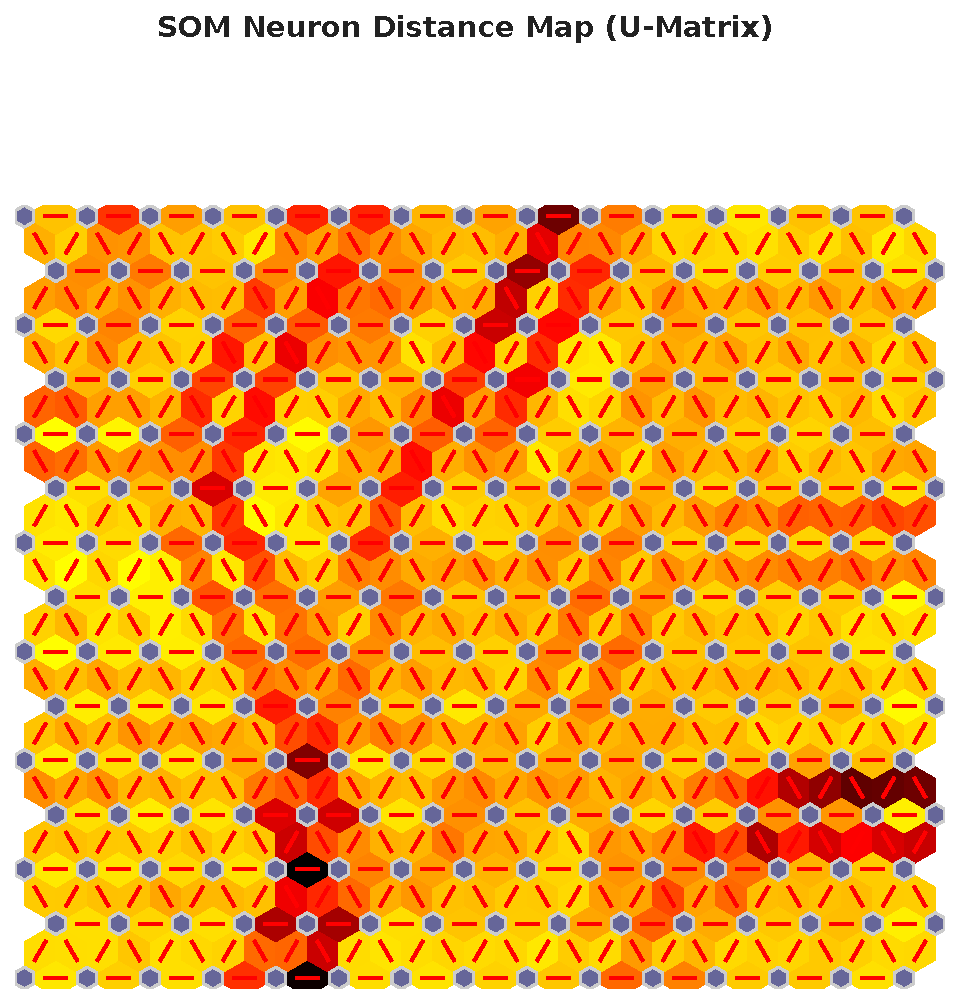
\includegraphics[width=\linewidth,keepaspectratio]{p2_u_matrix.pdf}
\end{minipage}\hfill
\begin{minipage}[c]{0.58\textwidth}\centering
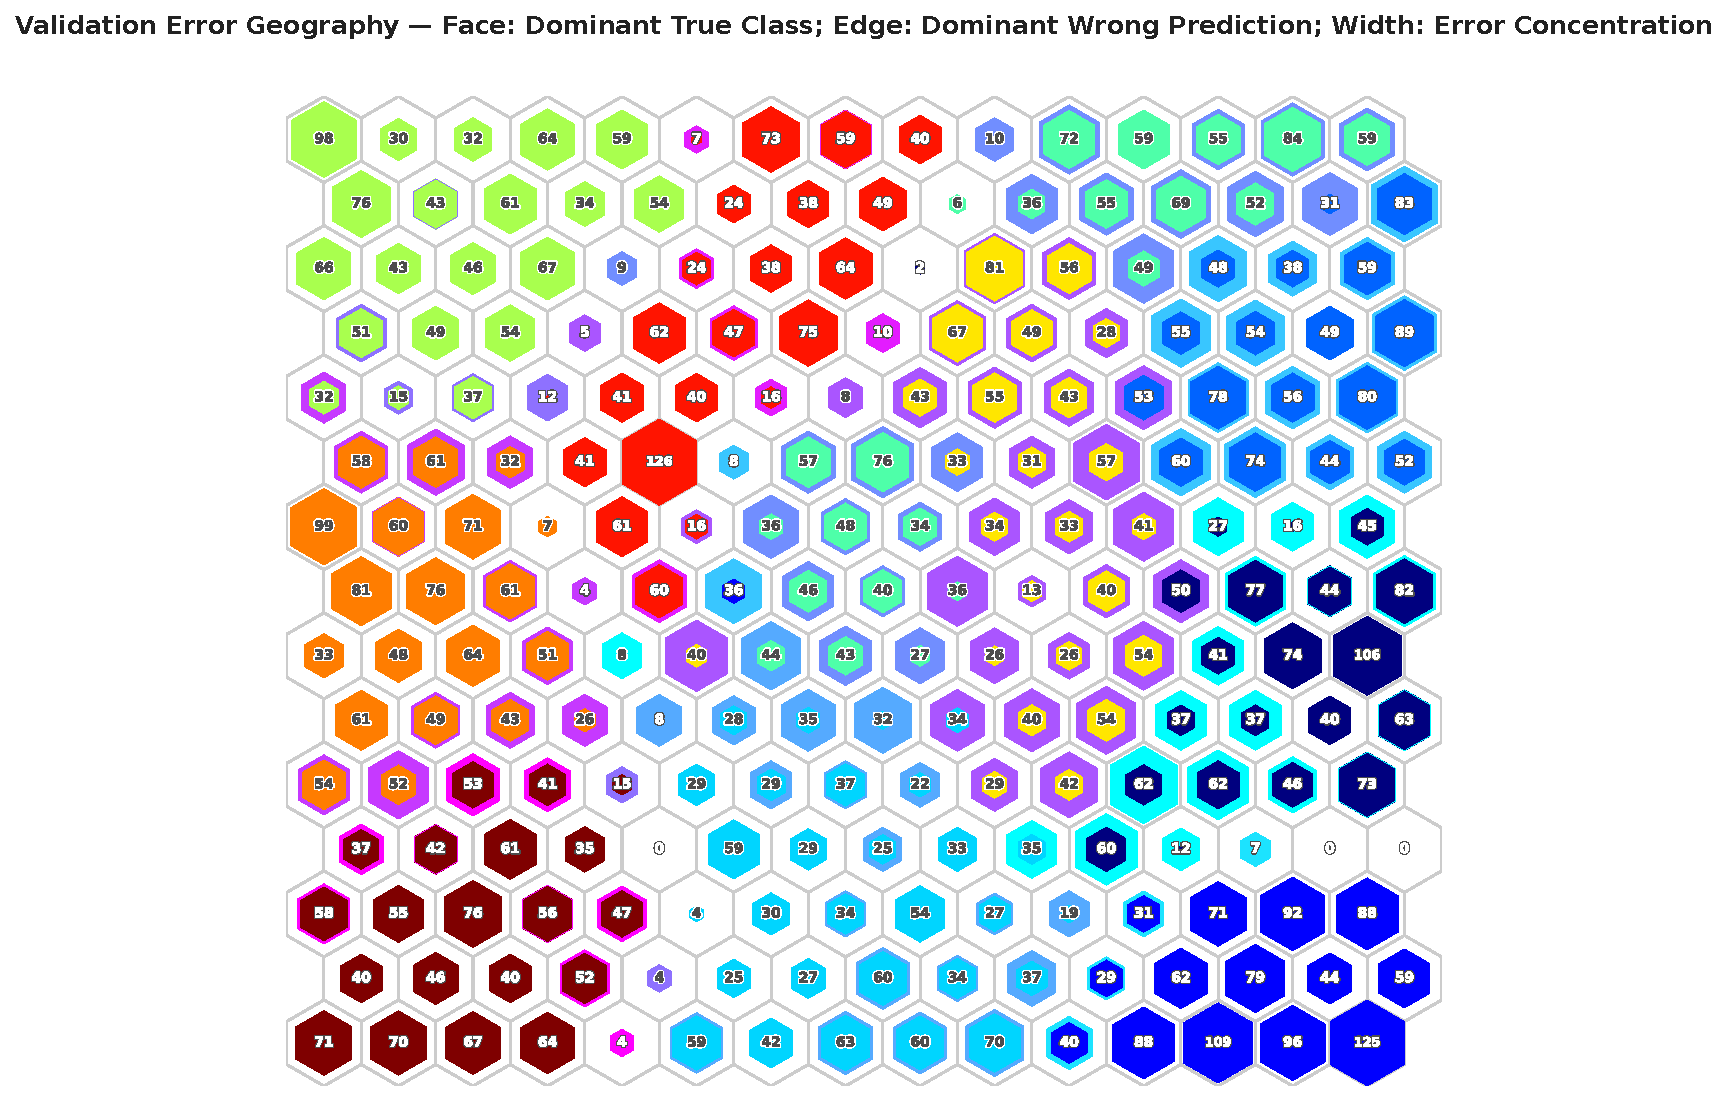
\includegraphics[width=\linewidth,keepaspectratio]{p2_validation_complex_error_map.pdf}
\end{minipage}
\caption{Left: U-matrix of the 15$\times$15 SOM (high values mark borders between groups of cells; the strongest borders surround the footwear). Right: validation error map (fill: most common true class; edge: most common wrong answer; size: how many mistakes). The mistakes fill the band where the upper-body garments meet.}
\label{fig:maps}
\end{figure}

\subsection{Comparison with baselines}

Table~\ref{tab:error-pattern-baselines} compares the SOM with the baselines on the same validation images. A SOM cell and a k-means cell find mistakes equally well (AUROC 0.811 and 0.812). Nearest-neighbour impurity does better (0.876), and the CNN's own confidence does best (0.906).
When every method flags the same 3.5\% of the images, the SOM catches 13.7\% of the mistakes and the confidence score 21.9\%. The gap is smaller than on MNIST (18\% against 53\%), because on Fashion-MNIST the network is often wrong without being unsure. The same-budget numbers are exploratory.

{\setlength{\tabcolsep}{3pt}\begin{table}[H]
\centering
\renewcommand{\arraystretch}{1.15}
\small
\begin{tabular}{|>{\raggedright\arraybackslash}p{0.30\textwidth}|>{\raggedright\arraybackslash}p{0.19\textwidth}|>{\raggedright\arraybackslash}p{0.13\textwidth}|>{\raggedright\arraybackslash}p{0.11\textwidth}|>{\raggedright\arraybackslash}p{0.14\textwidth}|}
\hline
\textbf{Score} & \textbf{AUROC (95\% range)} & \textbf{Hotspot ratio} & \textbf{Images flagged} & \textbf{Mistakes caught} \\ \hline
SOM 15$\times$15 cell error rate & 0.811 (0.796--0.824) & 3.9 (3.2--4.4) & 3.5\% & 13.7\% \\ \hline
k-means, 225 clusters, cell error rate & 0.812 (0.805--0.821) & 4.0 (3.7--4.5) & 4.0\% & 15.8\% \\ \hline
kNN impurity ($k=15$) & 0.876 (0.864--0.888) & --$^\dagger$ & 3.5\%$^\dagger$ & 21.1\% (19.2--22.9)$^\dagger$ \\ \hline
CNN max-softmax probability & 0.906 (0.898--0.914) & --$^\dagger$ & 3.5\%$^\dagger$ & 21.9\% (19.8--24.1)$^\dagger$ \\ \hline
\end{tabular}
\caption{How well each score finds the 876 validation images that the CNN gets wrong (10,500 images in total). Hotspot ratio: share of mistakes divided by share of images in the hotspot cells, chosen on one half and measured on the other; chance is about 1 ($p=0.005$). $^\dagger$kNN impurity and max-softmax score each image and form no cells, so instead they flag the same share of images as the SOM's hotspots (3.5\%, the images with the highest scores); the share of mistakes caught has a bootstrap interval. This same-budget comparison is exploratory, as on MNIST.}
\label{tab:error-pattern-baselines}
\end{table}
}

\subsection{Phase 3: Novelty detection}\label{sec:p3results}

\textbf{Far novelty (Table~\ref{tab:novelty}).} The SOM's quantization error separates SVHN from Fashion-MNIST better than chance (AUROC 0.789, 95\% interval 0.783--0.796; label shuffles give 0.500), but far less well than on MNIST (0.981). Energy (0.982), max-softmax (0.884) and nearest-neighbour distance (0.864) all do better; the primary statement, that QE is competitive with max-softmax, is not met ($-0.094$, $-0.101$ to $-0.088$).
The fixed QE alarm does not work: it flags 3.0\% of the SVHN images and 5.1\% of the normal validation images, so it catches \emph{fewer} novel images than normal ones (MNIST: 96.2\%).
The reason is one simple feature: SVHN embeddings are much shorter (average length 8.5, against 20.7), and length alone separates the two sets almost perfectly (AUROC 0.995). QE follows length only weakly (Spearman $-0.29$; MNIST $-0.83$), so the length effect that helped QE on MNIST works against it here.
Isolation Forest again ranks SVHN as \emph{more} normal (0.266), and the autoencoder depends on input scaling (0.583 raw, 0.676 standardised).

The SOM's own contribution is where the novel images land (Figure~\ref{fig:overlay}). All 26,032 SVHN images fall on 42 of the 225 cells; two cells receive 89\% of them, and 91\% land in cells whose most common class is Bag. To the map, SVHN looks like a typical bag.

\textbf{Near novelty: unseen clothing classes.} Here the SOM does better than on MNIST. With 6 known and 4 unseen classes, QE detects the unseen classes in all 5 splits (AUROC 0.739 to 0.831) and \textbf{beats max-softmax in every split} (+0.046, 95\% interval $+0.034$ to $+0.057$; on MNIST inconclusive). Clothing classes look alike, so the network is often confidently wrong about an unseen class, while the map still places it away from the known prototypes. Plain nearest-neighbour distance beats QE in every split ($-0.048$), so the 225 cells lose some detail.

\begin{table}[H]
\centering
\renewcommand{\arraystretch}{1.12}
\small
\begin{tabular}{|l|c|c|c|}
\hline
\textbf{Novelty score} & \textbf{AUROC} & \textbf{AUPR} & \textbf{FPR at 95\% TPR} \\ \hline
Energy & 0.982 & 0.988 & 0.063 \\ \hline
Maximum softmax probability & 0.884 & 0.936 & 0.307 \\ \hline
Nearest-neighbor distance ($k=5$) & 0.864 & 0.898 & 0.314 \\ \hline
SOM U-matrix score & 0.812 & 0.892 & 0.253 \\ \hline
SOM quantization error & 0.789 & 0.825 & 0.420 \\ \hline
One-Class SVM & 0.734 & 0.811 & 0.634 \\ \hline
Mahalanobis distance & 0.713 & 0.768 & 0.454 \\ \hline
Autoencoder (standardised inputs) & 0.676 & 0.768 & 0.653 \\ \hline
Autoencoder (raw inputs) & 0.583 & 0.702 & 0.744 \\ \hline
Isolation Forest & 0.266 & 0.564 & 0.934 \\ \hline
\end{tabular}
\caption{Far novelty with 10,500 Fashion-MNIST validation images as normal data and 26,032 SVHN test images as novel data (one network, one map, seed 42). AUPR treats SVHN as positive; its chance level is 0.713. A random score gives AUROC 0.505. The classical detectors (last five rows except Mahalanobis) are exploratory, as on MNIST.}
\label{tab:novelty}
\end{table}

\begin{figure}[H]
\centering
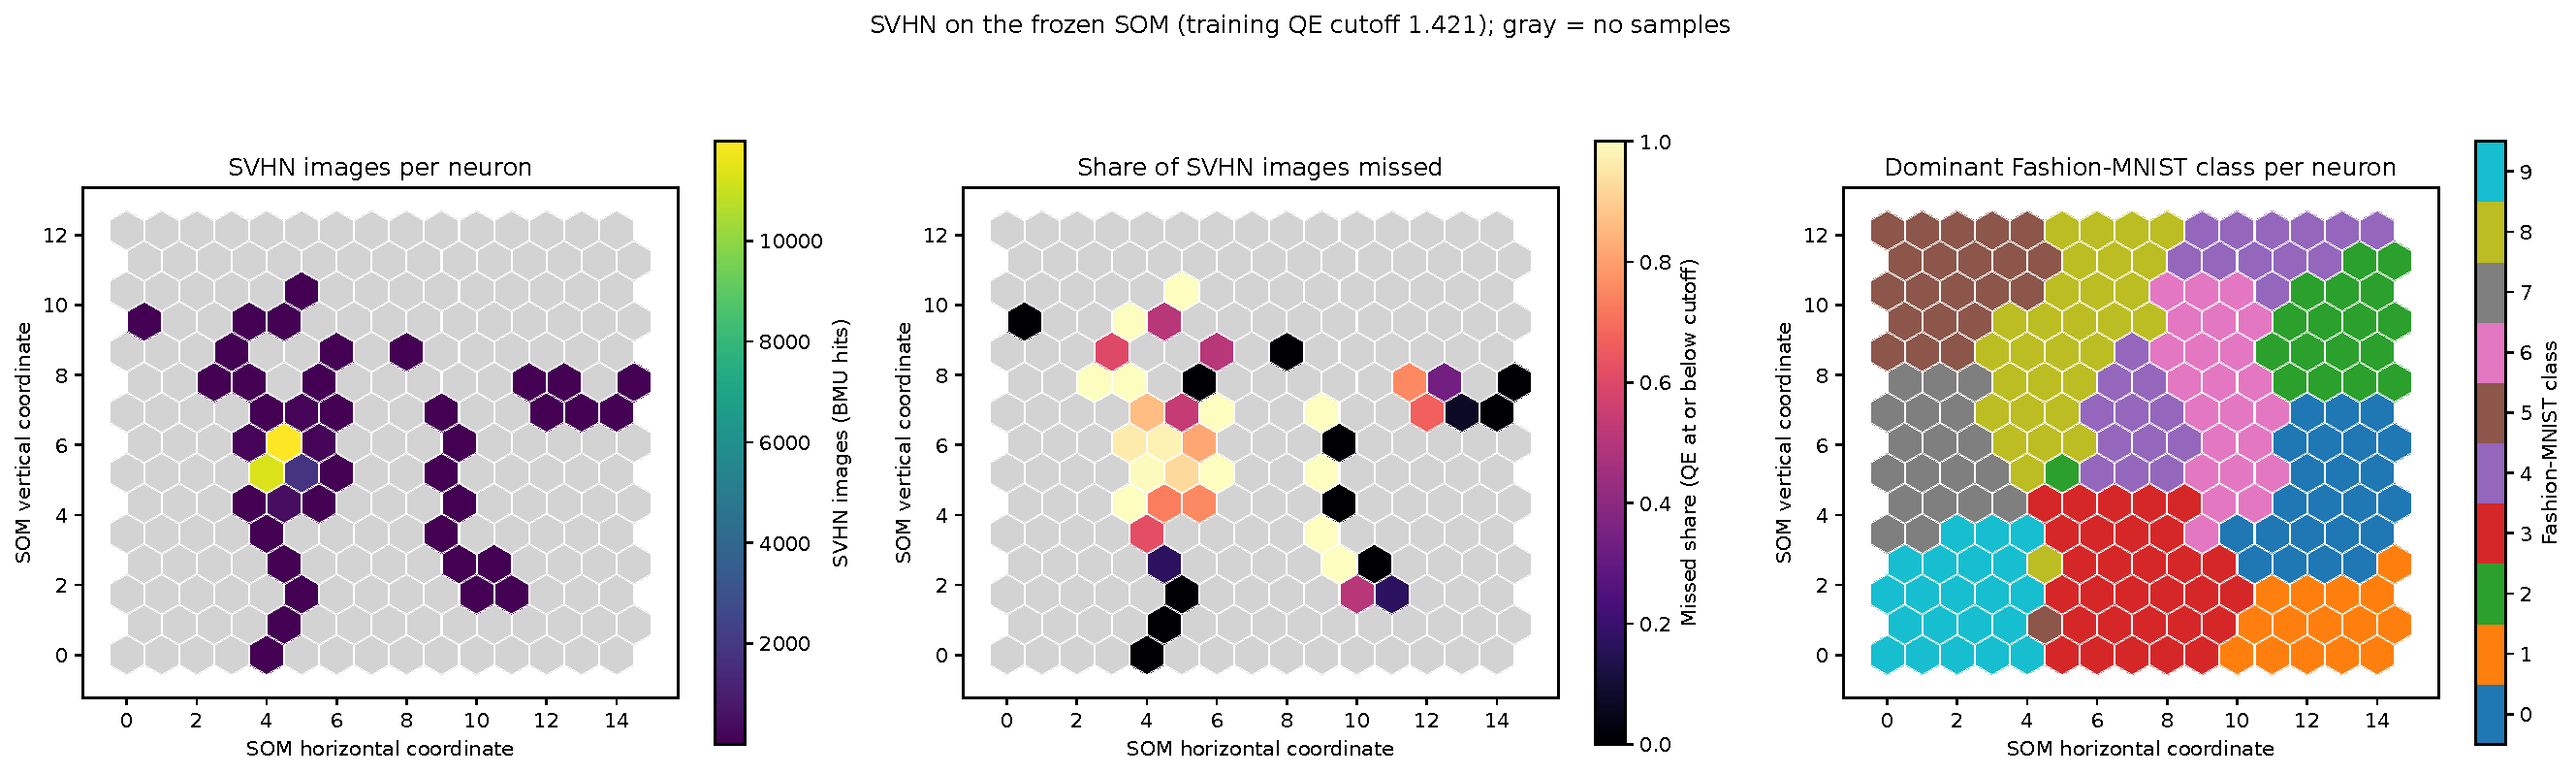
\includegraphics[width=0.95\textwidth,keepaspectratio]{p3_svhn_som_overlay.pdf}
\caption{Where the SVHN test images land on the 15$\times$15 SOM: images per cell (left), the share missed at the threshold, and the most common Fashion-MNIST class of each cell. Descriptive only.}
\label{fig:overlay}
\end{figure}

\subsection{Phase 4: Guided retraining}\label{sec:p4results}

Table~\ref{tab:retraining} gives the main results. \textbf{Targeted augmentation did not clearly help.} The SOM-guided arm lowered the error on the 422 test images in the hotspots from 36.0\% to 34.0\% (about 152 against 143 wrong), but the drop is not clear against normal training ($-2.0$ points, 95\% interval $-4.8$ to $+0.7$) or against the same number of random images ($-1.0$ points, $-3.2$ to $+1.1$). The primary criterion is \textbf{not met}; on MNIST it was met. Overall accuracy did not change (90.62\% against 90.66\%), and a rise of the error outside the hotspots of up to 0.37 points cannot be ruled out.
Two conditions, both fixed before the test, limit this test: the copies had to be altered four times less than on MNIST, and the hard pool covers 41\% of the training images, so it is far less selective and overlaps a random pool with the same class mix much more.

\textbf{The SOM was not a better picker than confidence.} The least-confident images gave a result that cannot be told apart from the SOM-guided arm ($-1.2$ points, $-3.3$ to $+0.8$), and adding the copies gradually made no clear difference. Per class, SOM-guided copies (mostly upper-body garments) lowered the Shirt error by 2.3 points but raised T-shirt/top, Dress and Bag: they moved the Shirt/T-shirt boundary more than they removed errors.

\textbf{Curriculum learning hurt, more than on MNIST.} The curriculum CNNs reached 87.37\% (SOM order), 89.15\% (random order) and 87.07\% (least-confident order), against 90.66\% for normal training; all three are clearly worse. The schedule only ever uses 40\% of the hard pool, so the hardest 60\% is never trained on: about a quarter of all training images here, against about 5\% on MNIST.
Forgetting was not a problem: in every arm the largest one-epoch drop in validation accuracy was 0.9 points or less, and every arm ended within 0.3 points of its best epoch.

\begin{table}[H]
\centering
\renewcommand{\arraystretch}{1.12}
\small
\begin{tabular}{|p{0.26\textwidth}|C{0.10\textwidth}|C{0.10\textwidth}|C{0.12\textwidth}|C{0.09\textwidth}|C{0.13\textwidth}|}
\hline
 & \multicolumn{2}{c|}{\textbf{Test images}} & \multicolumn{2}{c|}{\textbf{New SOM (validation)}} & \textbf{SVHN} \\ \hline
\textbf{Selection of hard images} & \textbf{Accuracy (\%)} & \textbf{Hotspot error (\%)} & \textbf{Hotspot error rate} & \textbf{Purity} & \textbf{QE AUROC} \\ \hline
None (normal training, CF1) & 90.66 & 36.0 & 0.406 & 0.884 & 0.838 \\ \hline
Random (augmentation) & 90.60 & 35.0 & 0.437 & 0.880 & 0.744 \\ \hline
Least confident (augmentation) & 90.57 & 35.2 & 0.413$^\dagger$ & 0.874$^\dagger$ & n/a \\ \hline
SOM-guided (augmentation, CF2) & 90.62 & 34.0 & 0.405 & 0.875 & 0.715 \\ \hline
SOM-guided (curriculum) & 87.37 & 51.8 & n/a & n/a & n/a \\ \hline
\end{tabular}
\caption{Retraining results, mean over 5 seeds. Test columns: accuracy on all 10,500 test images and error on the 422 test images in the hotspots. New SOM columns: error rate in the 11 worst cells and purity of a new 15$\times$15 SOM trained on each retrained CNN, on validation images. Last column: the new SOM's QE AUROC for SVHN against Fashion-MNIST validation images (Phase 1 network: 0.789). $^\dagger$From a secondary run added as on MNIST. n/a: not part of that run. The Phase 1 model (90.90\%) is a single run and is not in this table.}
\label{tab:retraining}
\end{table}

\textbf{What the new maps show.} The new SOMs after SOM-guided augmentation are not purer than after normal training (0.875 against 0.884), and their hotspots hold the same share of mistakes (0.405 against 0.406). Against random augmentation the hotspot error rate is lower (0.405 against 0.437, lower in all 5 seeds), but only because random augmentation made the weak regions worse. The topographic error rose (by 0.8 points, upper end of the interval 1.8, above the 1.0 limit), so the new maps may be less well ordered. Figure~\ref{fig:reanalysis} shows each seed. On MNIST the new maps had smaller weak regions than after normal training; here they do not.

\textbf{Novelty after retraining.} Every retrained network's SOM still detects SVHN better than chance (QE AUROC 0.59 to 0.93), but SOM-guided retraining \emph{lowered} it compared with normal training ($-0.123$, 95\% interval $-0.151$ to $-0.094$, lower in all 5 seeds), and the gap to max-softmax widened ($-0.100$). On MNIST retraining left it unchanged. Single networks vary a lot (0.728 to 0.935 for normal training alone), which is why the comparison is paired by seed.

\begin{figure}[H]
\centering
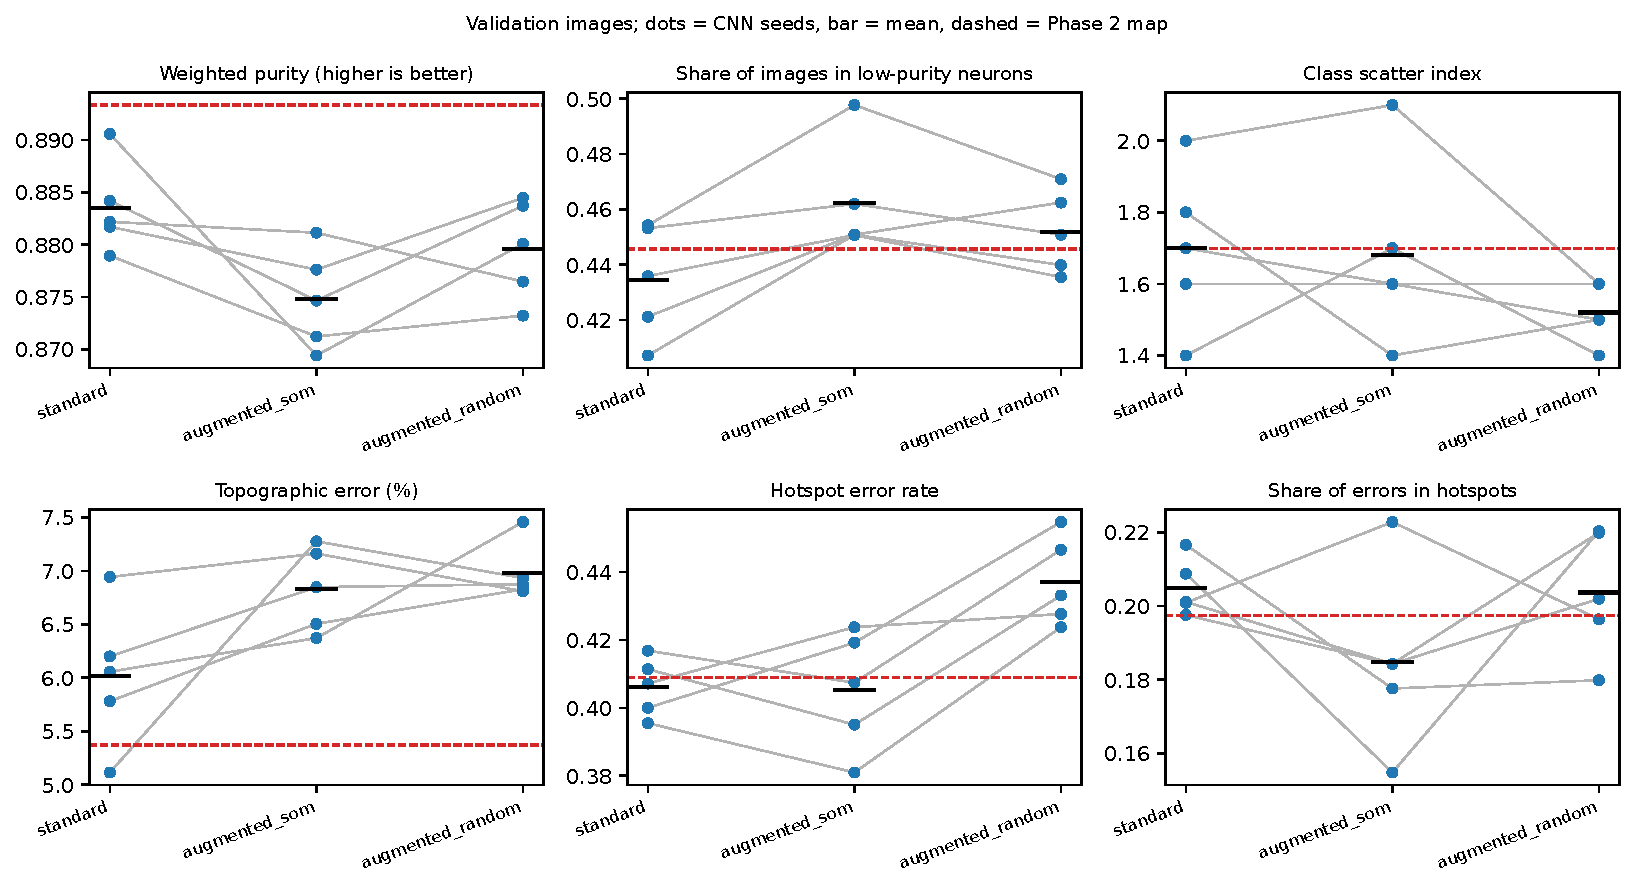
\includegraphics[width=\textwidth]{p4_map_measures_by_arm.pdf}
\caption{Measures of the new SOMs on validation images. Each dot is one CNN seed, the black bar is the mean over seeds, and the dashed line is the Phase 2 map.}
\label{fig:reanalysis}
\end{figure}

\subsection{End-to-end comparison}

Figure~\ref{fig:cf} shows CF1 (normal training), CF2 (SOM-guided augmentation) and their difference on the same 10,500 test images, averaged over 5 seeds. The clearest changes are on the Shirt and T-shirt/top classes: more shirts are right and fewer are called T-shirts, while more T-shirts are called shirts.
Net, CF2 has about the same number of mistakes as CF1 (985.2 against 980.6 on average); on the 422 hotspot images it has about 8 fewer (143.4 against 151.8), fewer in 4 of the 5 seeds. Individual mistakes move a lot: for each seed the SOM-guided CNN fixes about 335 of the standard CNN's mistakes and makes about 340 new ones, and the net change over all images ranges from $-49$ to $+69$ between seeds. We therefore read the end-to-end effect as no gain overall and, at most, a small and uncertain gain on the hotspots.

\begin{figure}[H]
\centering
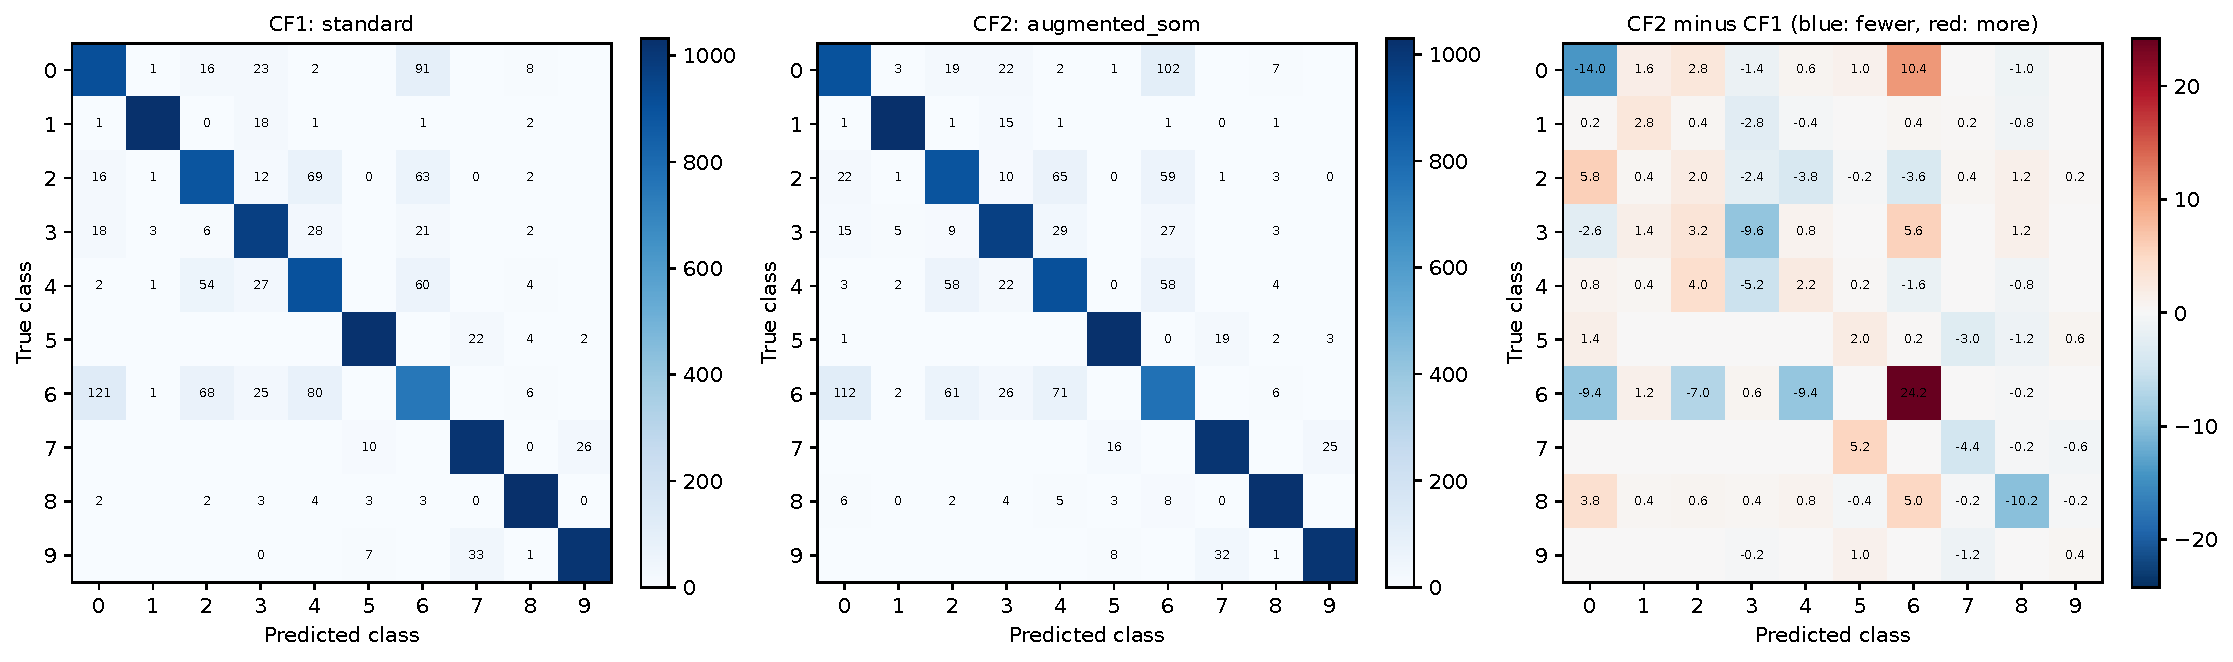
\includegraphics[width=\textwidth]{p4_confusion_standard_vs_augmented_som.pdf}
\caption{CF1 (normal training) and CF2 (SOM-guided augmentation): mean test confusion matrices over 5 seeds, and their difference (blue: fewer cases, red: more). Classes: 0 T-shirt/top, 1 Trouser, 2 Pullover, 3 Dress, 4 Coat, 5 Sandal, 6 Shirt, 7 Sneaker, 8 Bag, 9 Ankle boot.}
\label{fig:cf}
\end{figure}

\subsection{Fashion-MNIST next to MNIST}

\begin{table}[H]
\centering
\renewcommand{\arraystretch}{1.12}
\footnotesize
\begin{tabular}{|>{\raggedright\arraybackslash}p{0.44\textwidth}|C{0.22\textwidth}|C{0.22\textwidth}|}
\hline
\textbf{Result} & \textbf{Fashion-MNIST} & \textbf{MNIST} \\ \hline
Test accuracy of the baseline CNN & 90.90\% & 99.18\% \\ \hline
SOM purity (shuffled labels) & 89.3\% (17.3\%) & 98.2\% (17.4\%) \\ \hline
Hotspot concentration ratio (chance about 1) & 3.9 & 11.1 \\ \hline
Spearman, cell error rate vs.\ purity & $-0.95$ & $-0.81$ \\ \hline
Grid comparison, 20$\times$20 vs 15$\times$15 & 15$\times$15 better & inconclusive \\ \hline
Mistake finding AUROC: SOM / k-means / max-softmax & 0.811 / 0.812 / 0.906 & 0.685 / 0.693 / 0.981 \\ \hline
SVHN: SOM QE / energy AUROC & 0.789 / 0.982 & 0.981 / 0.9998 \\ \hline
SVHN caught by the fixed QE alarm & 3.0\% & 96.2\% \\ \hline
Unseen classes: QE minus max-softmax & +0.046, QE better & inconclusive \\ \hline
A1: SOM copies beat random copies on hotspots & $-1.0$ points, not met & $-2.5$ points, met \\ \hline
Curriculum vs normal training & worse (3.3 points) & worse (0.45 points) \\ \hline
New SOM hotspots smaller than after normal training & no & yes \\ \hline
SOM-guided retraining and novelty AUROC & lowered & unchanged \\ \hline
\end{tabular}
\caption{The same design on both datasets. MNIST values are from the MNIST final and phase reports.}
\label{tab:mnist}
\end{table}

\section{Discussion and Limitations}

On Fashion-MNIST the SOM again turns the 84-number embeddings into a readable map: footwear, trousers and bags form clean regions, and the upper-body garments share one mixed region where the mistakes gather, far beyond chance and on three grid sizes. The kind of failure differs from MNIST. There, a few small cells held unusual handwriting; here, whole classes overlap, so the map's value is to show \emph{which group of classes} the network cannot separate.
As on MNIST, the map is not the best mistake finder: k-means does as well and the CNN's confidence does better.

For novelty the picture is mixed. Against far novelty (SVHN) the SOM is weak and its fixed alarm fails, because SVHN differs mainly in embedding length and the map sees it as a bag. Against near novelty (unseen clothing classes), the case closer to real use, it beats the CNN's confidence in every split, which it did not do on MNIST. Nearest-neighbour distance does better still.

Guided retraining, which helped on MNIST, did not carry over. The SOM-chosen copies did not clearly lower the hotspot error, did not change overall accuracy, did not make the new maps cleaner and lowered the map's novelty signal. Curriculum learning hurt on both datasets. The more errors there are to fix, the less a rule designed on MNIST picks out a useful subset: the hard pool grew from 8.6\% to 41\% of the training images.

\textbf{Limitations.}
(1)~One network and one SOM seed for the headline Phase 2 and Phase 3 results; the SOM seed alone moves the SVHN AUROC by about 0.1.
(2)~Every setting was copied from MNIST and not tuned for Fashion-MNIST, by design. A pool rule or curriculum schedule chosen for this dataset, under a new protocol, could give a fairer test of SOM guidance.
(3)~The augmentation had to be four times weaker than on MNIST, which leaves it less room to help.
(4)~SVHN is the only outside set and differs mainly in embedding length; near novelty is covered only by unseen Fashion-MNIST classes, and those splits share classes.
(5)~In Phase 4 the hotspots come from the SOM, which favours the SOM-guided arms on hotspot error, the pools come from one SOM, and five seeds can only separate fairly large differences.
(6)~The baseline comparison, the same-budget check and the length diagnostics are exploratory, and the validation images were also used to choose the CNN checkpoint.

\section{Conclusion}

On Fashion-MNIST, a SOM trained on a CNN's embeddings shows where the CNN's mistakes gather: in a broad region where upper-body garments overlap, about four times more than chance. It does not find mistakes better than k-means or the CNN's confidence. As a novelty detector it is weak against SVHN but beats the CNN's confidence on clothing classes the network never saw.
Using its hotspots to guide retraining, which worked on MNIST, gave no clear gain here, and curriculum learning made the CNN worse on both datasets. Across the two datasets the SOM is most useful as an \emph{explainer}, showing where and between which classes a network fails, rather than as a selector of training images.
The next steps are to test a pool rule and schedule chosen for Fashion-MNIST under a new protocol, and to repeat the near-novelty test on the retrained networks.

\clearpage
\printbibliography[title={References}]

\end{document}
